\setcounter{chapter}{1}
\chapter{Univariate Random Variable}
\makeheading{Lecture 1 | 2020-09-09}
Review probability model, random variable (r.v.),
expectation, and moment generating function.

\section{Probability Model and Random Variable}
\begin{Definition}{Probability model}{}
    A \textbf{probability model} is used for a random
    experiment. It has three important components:
    \begin{enumerate}[label=(\Roman*)]
        \item Sample space
        \item Event
        \item Probability function
    \end{enumerate}
\end{Definition}

\begin{Definition}{Sample space}{}
    A \textbf{sample space} $ S $ is
    the collection of all possible outcomes of one single
    random experiment.
\end{Definition}
\begin{Definition}{Event}{}
    An \textbf{event} $ A,B,\ldots $ is a subset of $ S $.
\end{Definition}

\begin{Example}{}{}
    Toss a coin twice.
    \begin{itemize}
        \item $ S=\set{(H,H),(H,T),(T,H),(T,T)} $
        \item $ A $: First toss is a head $ (H) $.
    \end{itemize}
    Clearly, $ A=\set{(H,H),(H,T)}\subseteq S $, so $ A $ is an event.
\end{Example}

\begin{Definition}{Probability function}{psf_def}
    A \textbf{probability function} $ \Prob{} $
    is a function of events and satisfies:
    \begin{enumerate}[label=(\Roman*)]
        \item\label{psf_def_1} For any event $ A $, $ \Prob{A}\ge 0 $
        \item\label{psf_def_2} $ \Prob{S}=1 $
        \item\label{psf_def_3} \emph{Additivity property}: If $ A_1,A_2,A_3,\ldots $
              are pairwise mutually exclusive events; that is, $ A_i\cap A_j=\varnothing $
              for all $ i\neq j $, then
              \[ \Prob[\bigg]{\bigcup_{i=1}^{\infty}A_i}=\sum\limits_{i=1}^{\infty} \Prob{A_i} \]
    \end{enumerate}
\end{Definition}

\begin{Example}{}{}
    Toss a coin twice, given one event $ A $,
    \[ \Prob{A}=\frac{\text{\# of outcomes in }A}{4}  \]
    where $ 4 $ is the total number of outcomes in $ S $.
    $ \Prob{} $ satisfies the three properties, therefore $ \Prob{} $ is a probability function.
\end{Example}

\begin{Proposition}{Additional Properties of the Probability Function}{add_prop_psf}
    \begin{enumerate}[label=(\arabic*)]
        \item\label{add_prop_psf_1} $ \Prob{\varnothing}=0 $
              where $ \varnothing=\bigcup_{i=1}^\infty \varnothing $.
        \item\label{add_prop_psf_2} Let $ \bar{A} $
              be the complementary event of $ A $.
              \begin{enumerate}[label=(\roman*)]
                  \item $ \bar{A}\cup A=S $
                  \item $ \bar{A}\cap A=\varnothing $
                        \[ \Prob{A}+\Prob{\bar{A}}=1 \]
              \end{enumerate}
        \item If $ A_1 $ and $ A_2 $ are mutually exclusive, then
              \[ \Prob{A_1\cup A_2}=\Prob{A_1}+\Prob{A_2}. \]
        \item\label{add_prop_psf_3} Generally,
              \[ \Prob{A_1\cup A_2}=\Prob{A_1}+\Prob{A_2}-
                  \Prob{A_1\cap A_2} \]
              \begin{center}
                  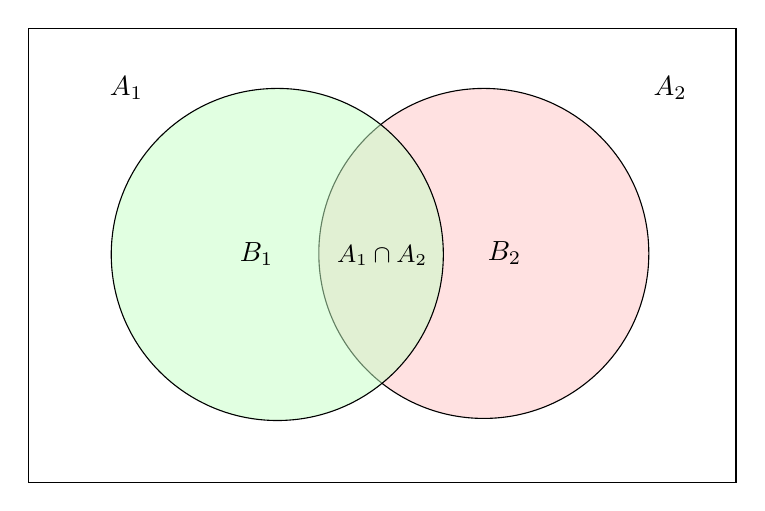
\begin{tikzpicture}[x=0.75pt,y=0.75pt,yscale=-1,xscale=1]
                      %Shape: Circle [id:dp45613176616869144] 
                      \draw  [fill={rgb, 255:red, 255; green, 196; blue, 196 }  ,fill opacity=0.5 ] (148.67,117.83) .. controls (148.67,73.93) and (184.26,38.33) .. (228.17,38.33) .. controls (272.07,38.33) and (307.67,73.93) .. (307.67,117.83) .. controls (307.67,161.74) and (272.07,197.33) .. (228.17,197.33) .. controls (184.26,197.33) and (148.67,161.74) .. (148.67,117.83) -- cycle ;
                      %Shape: Circle [id:dp3007887211930459] 
                      \draw  [fill={rgb, 255:red, 196; green, 255; blue, 196 }  ,fill opacity=0.5 ]  (48.67,118.33) .. controls (48.67,74.15) and (84.48,38.33) .. (128.67,38.33) .. controls (172.85,38.33) and (208.67,74.15) .. (208.67,118.33) .. controls (208.67,162.52) and (172.85,198.33) .. (128.67,198.33) .. controls (84.48,198.33) and (48.67,162.52) .. (48.67,118.33) -- cycle ;
                      %Shape: Rectangle [id:dp5844224741640769] 
                      \draw   (8.67,9.33) -- (349.67,9.33) -- (349.67,228.33) -- (8.67,228.33) -- cycle ;
                      % Text Node
                      \draw (65.23,44.98) node [anchor=south east] [inner sep=0.75pt]    {$A_{1}$};
                      % Text Node
                      \draw (327.23,44.98) node [anchor=south east] [inner sep=0.75pt]    {$A_{2}$};
                      % Text Node
                      \draw (118.67,118.33) node    {$B_{1}$};
                      % Text Node
                      \draw (238.17,117.83) node    {$B_{2}$};
                      % Text Node
                      \draw (179.17,118.83) node  [font=\small]  {$A_{1} \cap A_{2}$};
                  \end{tikzpicture}
              \end{center}
              \[ A_1\cup A_2=B_1\cup (A_1\cap A_2)\cup B_2 \]
        \item If $ A_1\subseteq A_2 $, then $ \Prob{A_1}\le \Prob{A_2} $.
              \begin{center}
                  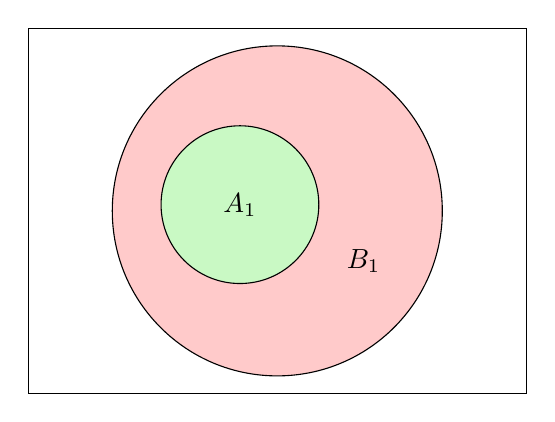
\begin{tikzpicture}[x=0.75pt,y=0.75pt,yscale=-1,xscale=1]
                      %Shape: Circle [id:dp45613176616869144] 
                      \draw  [fill={rgb, 255:red, 255; green, 196; blue, 196 }  ,fill opacity=0.9 ] (49.17,97.33) .. controls (49.17,53.43) and (84.76,17.83) .. (128.67,17.83) .. controls (172.57,17.83) and (208.17,53.43) .. (208.17,97.33) .. controls (208.17,141.24) and (172.57,176.83) .. (128.67,176.83) .. controls (84.76,176.83) and (49.17,141.24) .. (49.17,97.33) -- cycle ;
                      %Shape: Circle [id:dp3007887211930459] 
                      \draw  [fill={rgb, 255:red, 196; green, 255; blue, 196 }  ,fill opacity=0.9 ] (72.67,94.33) .. controls (72.67,73.35) and (89.68,56.33) .. (110.67,56.33) .. controls (131.65,56.33) and (148.67,73.35) .. (148.67,94.33) .. controls (148.67,115.32) and (131.65,132.33) .. (110.67,132.33) .. controls (89.68,132.33) and (72.67,115.32) .. (72.67,94.33) -- cycle ;
                      %Shape: Rectangle [id:dp5844224741640769] 
                      \draw   (8.67,9.33) -- (248.67,9.33) -- (248.67,185.33) -- (8.67,185.33) -- cycle ;
                      % Text Node
                      \draw (110.67,94.33) node    {$A_{1}$};
                      % Text Node
                      \draw (179.58,128.12) node [anchor=south east] [inner sep=0.75pt]    {$B_{1}$};
                  \end{tikzpicture}
              \end{center}
              \[ A_2=A_1\cup B_1 \]

    \end{enumerate}
\end{Proposition}
\begin{Proof}{\ref{prop:add_prop_psf}}{}
    Proof of~\ref{add_prop_psf_1}: Let $ A_1=\varnothing $, $ A_2=\varnothing $,
    $ A_3=\varnothing $, $ \ldots $, then
    \[ \Prob{\varnothing}=
        \Prob[\bigg]{\bigcup_{i=1}^\infty A_i}=
        \sum_{i=1}^{n} \Prob{A_i}=\sum_{i=1}^{n}\Prob{\varnothing} \]

\end{Proof}
\begin{Definition}{Conditional probability}{}
    Suppose $ A $ and $ B $ are two events with
    $ \Prob{B}>0 $. The \textbf{conditional probability}
    of $ A $ given that $ B $ is
    \[ \Prob{A\given B}=\frac{\Prob{A\cap B}}{\Prob{B}} \]
\end{Definition}

\begin{Definition}{Independent events}{}
    Suppose $ A $ and $ B $ are two events. $ A $ and
    $ B $ are \textbf{independent events} if and only if
    \[ \Prob{A\cap B}=\Prob{A}\Prob{B} \]
\end{Definition}

Clearly, $ \Prob{A\given B}=\Prob{A} $ if and only if $ A $ and $ B $ are independent since
\[ \Prob{A\given B}=\frac{\Prob{A\cap B}}{\Prob{B}}=\frac{\Prob{A}\Prob{B}}{\Prob{B}}=\Prob{A}  \]

\begin{Example}{}{}
    Toss a coin twice.
    \begin{itemize}
        \item $ A $: First toss is $ H $
        \item $ B $: Second toss is $ T $
    \end{itemize}
    \[ \Prob{A}=\frac{\text{\# of outcomes in }A}{4}=\frac{2}{4}\quad
        \text{ and }\quad \Prob{B}=\frac{2}{4} \]
    \[ \Prob{A\cap B}=\frac{1}{4}=\Prob{A}\Prob{B} \]
    Therefore, $ A $ and $ B $ are independent.
\end{Example}

\begin{Definition}{Random variable}{}
    A \textbf{random variable} (r.v.) $ X $
    is a function from a sample space $ S $ to the real numbers $ \mathbf{R} $; that is,
    \[ X:S\to \mathbf{R} \] satisfies for any given $ x\in\mathbf{R} $
    $ \set{X\le x} $ is an event.
    \[ \set{X\le x}=\set{w\in S:X(w)\le x}
        \subseteq S \]
\end{Definition}

\begin{Example}{}{}
    Toss a coin twice. Let $ X $ be the number of heads $ (H) $ in two tosses.
    Verify that $ X $ is a random variable.

    \textbf{Solution.}
    Possible values of $ X $: $ 0,1,2 $. Given $ x\in\mathbf{R} $,
    $ \set{X\le x} $.
    \begin{itemize}
        \item $ x<0 \implies \set{X\le x}=\varnothing $
        \item $ x=0 \implies \set{X\le x}=\set{X=0}=\set{(T,T)}\subseteq S$
        \item $ x=1 \implies \set{X\le x}=\set{X=1}=\set{(H,T),(T,H)}
                  \subseteq S $
        \item $ x=2 \implies \set{X\le x}=\set{X=2}=
                  \set{(H,H)}\subseteq S $
    \end{itemize}
    Thus, $ X $ is a random variable.
\end{Example}

\begin{Definition}{Cumulative distribution function}{}
    The \textbf{cumulative distribution function} (c.d.f.) of a random variable
    $ X $ is defined by
    \[ F(x)=\Prob{X\le x}\quad\text{for all $ x\in\mathbf{R} $} \]
    Note that the c.d.f.\ is defined for all $ \mathbf{R} $.
\end{Definition}

\begin{Definition}{Properties --- Cumulative Distribution Function}{}
    \begin{enumerate}[label=(\arabic*)]
        \item $ F $ is a non-decreasing function; that is, if $ x_1\le x_2 $,
              then $ F(x_1)\le F(x_2) $.

              By looking at:
              \begin{itemize}
                  \item $ \set{X\le x_1}\subseteq \set{X\le x_2} $
                        if $ x_1\le x_2 $.
              \end{itemize}
        \item $ \lim\limits_{{x} \to {\infty}} F(x)=1 $
              and $ \lim\limits_{{x} \to {-\infty}} F(x)=0 $.

              By looking at:
              \begin{itemize}
                  \item $ \set{X\le x} \to S $ as $ x\to\infty $.
                  \item $ \set{X\le x} \to \varnothing $ as $ x\to-\infty $.
              \end{itemize}
        \item $ F(x) $ is a right continuous function; that is,
              for any $ a\in\mathbf{R} $,
              \[ \lim\limits_{{x} \to {a^+}} F(x)=F(a) \]
    \end{enumerate}
\end{Definition}
\begin{figure}[!ht]
    \centering
    \begin{tikzpicture}[x=0.75pt,y=0.75pt,yscale=-1,xscale=1]
        %Curve Lines [id:da10991679289562262] 
        \draw    (22.67,142.17) .. controls (62.67,112.17) and (163.67,135.17) .. (202.67,100.17) ;
        %Curve Lines [id:da07899179356252228] 
        \draw    (202.67,55.5) .. controls (242.67,25.5) and (357.67,48.5) .. (392.67,11.5) ;
        %Shape: Circle [id:dp5581982780608664] 
        \draw   (194.83,92.33) .. controls (194.83,88.01) and (198.34,84.5) .. (202.67,84.5) .. controls (206.99,84.5) and (210.5,88.01) .. (210.5,92.33) .. controls (210.5,96.66) and (206.99,100.17) .. (202.67,100.17) .. controls (198.34,100.17) and (194.83,96.66) .. (194.83,92.33) -- cycle ;
        %Shape: Circle [id:dp6983301165229509] 
        \draw  [fill={rgb, 255:red, 0; green, 0; blue, 0 }  ,fill opacity=1 ] (194.83,63.33) .. controls (194.83,59.01) and (198.34,55.5) .. (202.67,55.5) .. controls (206.99,55.5) and (210.5,59.01) .. (210.5,63.33) .. controls (210.5,67.66) and (206.99,71.17) .. (202.67,71.17) .. controls (198.34,71.17) and (194.83,67.66) .. (194.83,63.33) -- cycle ;
        %Straight Lines [id:da8561892708640969] 
        \draw    (12,161) -- (424.67,161.33) ;
        %Straight Lines [id:da40985872868130113] 
        \draw    (202.67,154.33) -- (202.67,168.33) ;
        \draw    (405.17,140.33) -- (203.67,140.33) ;
        \draw [shift={(201.67,140.33)}, rotate = 360] [color={rgb, 255:red, 0; green, 0; blue, 0 }  ][line width=0.75]    (10.93,-3.29) .. controls (6.95,-1.4) and (3.31,-0.3) .. (0,0) .. controls (3.31,0.3) and (6.95,1.4) .. (10.93,3.29)   ;

        % Text Node
        \draw (202.67,171.73) node [anchor=north] [inner sep=0.75pt]    {$a$};
    \end{tikzpicture}
    \caption{Right Continuous}
\end{figure}
\begin{figure}[!ht]
    \centering
    \begin{tikzpicture}[x=0.75pt,y=0.75pt,yscale=-1,xscale=1]
        %uncomment if require: \path (0,300); %set diagram left start at 0, and has height of 300

        %Curve Lines [id:da10991679289562262] 
        \draw    (22.67,142.17) .. controls (62.67,112.17) and (163.67,135.17) .. (202.67,100.17) ;
        %Curve Lines [id:da07899179356252228] 
        \draw    (202.67,55.5) .. controls (242.67,25.5) and (357.67,48.5) .. (392.67,11.5) ;
        %Shape: Circle [id:dp5581982780608664] 
        \draw  [fill={rgb, 255:red, 0; green, 0; blue, 0 }  ,fill opacity=1 ] (194.83,92.33) .. controls (194.83,88.01) and (198.34,84.5) .. (202.67,84.5) .. controls (206.99,84.5) and (210.5,88.01) .. (210.5,92.33) .. controls (210.5,96.66) and (206.99,100.17) .. (202.67,100.17) .. controls (198.34,100.17) and (194.83,96.66) .. (194.83,92.33) -- cycle ;
        %Shape: Circle [id:dp6983301165229509] 
        \draw   (194.83,63.33) .. controls (194.83,59.01) and (198.34,55.5) .. (202.67,55.5) .. controls (206.99,55.5) and (210.5,59.01) .. (210.5,63.33) .. controls (210.5,67.66) and (206.99,71.17) .. (202.67,71.17) .. controls (198.34,71.17) and (194.83,67.66) .. (194.83,63.33) -- cycle ;
        %Straight Lines [id:da8561892708640969] 
        \draw    (12,161) -- (424.67,161.33) ;
        %Straight Lines [id:da40985872868130113] 
        \draw    (202.67,154.33) -- (202.67,168.33) ;
        %Straight Lines [id:da9341376741643171] 
        \draw    (405.17,140.33) -- (203.67,140.33) ;
        \draw [shift={(201.67,140.33)}, rotate = 360] [color={rgb, 255:red, 0; green, 0; blue, 0 }  ][line width=0.75]    (10.93,-3.29) .. controls (6.95,-1.4) and (3.31,-0.3) .. (0,0) .. controls (3.31,0.3) and (6.95,1.4) .. (10.93,3.29)   ;

        % Text Node
        \draw (202.67,171.73) node [anchor=north] [inner sep=0.75pt]    {$a$};
    \end{tikzpicture}
    \caption{Not Right Continuous}
\end{figure}
\begin{Proposition}{Additional Properties of Cumulative Distribution Function}{}
    \begin{enumerate}[label=(\arabic*)]
        \item $ \Prob{a<X\le b}=\Prob{X\le b}-\Prob{X\le a}=F(b)-F(a) $
        \item $ \Prob{X=x}=\Prob{\text{Jump at $ x $}}=\lim\limits_{{t} \to {x^+}}
                  F(t)-\lim\limits_{{t} \to {x^-}}F(t)=F(x)-\lim\limits_{{t} \to {x^-}} F(t) $
    \end{enumerate}
\end{Proposition}
